% ch/maxwald.tex: sections of Chapter chap:maxwald, whose heading and opening are in ch/c14.tex.
\section{Notation}\label{mw:sec:notation}

The manuscript uses notation that differs from the book's in several places, and we convert throughout. Its Laplace variable $\lambda$ is kept here, and it is the variable $u$ of Section~\ref{ch:clock}, so that its $R(\lambda)=\xi(\frac12)/\xi(\frac12+\sqrt\lambda)$ is $1/G(\lambda)$ (written $\varphi_{1/2}$ when the basepoint family is in view) and its basepoint transforms $R_\alpha$ are the $\varphi_\alpha$ of Theorem~\ref{bp:thm:alpha}. Its reciprocal Xi law is the clock $T$, its heat trace $S(x)=\sum_{\Im\rho>0}e^{(\rho-1/2)^2x}$ is the function $W(x)$ of Section~\ref{ch:clock}, one term for each pair $\{\rho,1-\rho\}$ counted with multiplicity, its $\lambda_\rho=(\rho-\frac12)^2$ is $-a_\rho$, and its $\psi(\lambda)=\frac d{d\lambda}\log\xi(\frac12+\sqrt\lambda)$ is $(G'/G)(\lambda)$, because $\psi$ is the digamma function in the book. Its smoothed Thorin density $\rho_\varepsilon(x)=\pi^{-1}\Im\psi(-x-i\varepsilon)$ is written $r_\eta(x)=\pi^{-1}\Im(G'/G)(-x-i\eta)$, with $\eta>0$ the distance below the cut, because $\rho_\varepsilon(\theta)$ is the basepoint density of \eqref{eq:rho}; the relation between the two is in Section~\ref{ch:ggc}. Its L\'evy density $k(x)$ is $W(x)/x$, because the book's $k$ is $x$ times the L\'evy density, and its Bondesson class $\mathcal B$ is $\mathrm{BO}$. Its uniform variable $U$ and the space component $W$ of a Wald couple are written $\upsilon$ and $\varsigma$, because $U$ is the Thorin measure and $W$ the heat trace of the book. Its P\'olya kernel is $\Phi_{\mathrm{dBN}}(u)=\frac12\Phi(2u)$ of Section~\ref{ch:dbn}, so that $\Phi(u)=2\Phi_{\mathrm{dBN}}(u/2)$ for the kernel \eqref{eq:ch2:Phi} of the book, which is Titchmarsh's, and its P\'olya density $4\Phi_{\mathrm{dBN}}/\Xi(0)$ is the density of $V=X/2$, where $X$ has the density $p=\Phi/\Xi(0)$ of Section~\ref{ch:clock}. Its variable $Y$ with $\E Y^s=2\xi(s)$ is $e^Y$ for the variable $Y$ of the book, $\E e^{sY}=2\xi(s)$. Its maximum $M$ is $M_4$, and the independent copies $M_1$, $M_2$ in its $M_1+M_2$ are written $M_4$ and $M_4'$, because $M_1$ is another law in Section~\ref{sec:ch16:max}. Its $\theta$ and $\theta_4$ are $\vartheta$ and $\vartheta_4$, and its zeta distributed integer $N$ is $N_\sigma$. With these conversions its formula $\Phi_{\mathrm{dBN}}(u)=\frac14e^{3u}f(e^{2u})$ for the density $f$ of its $Y$ becomes $\Phi(u)=\frac12e^{3u/2}f(e^u)$ for the density $f$ of $e^Y$, which is Proposition~\ref{mw:prop:sum}(ii). The remaining conversions are made where the symbols occur: the manuscript's flow law $T_t$ has the transform $R_t(\lambda/2)$, with $R_t$ the flow transform of Section~\ref{ch:dbn}, so it is half of the flow clock; its approximant $T_H$ is the law with transform $1/G_N$ of Section~\ref{sec:weak:limits}; its residue coefficients $c_\rho$ are the $R_k=-\gamma_k^2c_k$ of Section~\ref{ch:clocklaw}; its density $u_\alpha$ of the basepoint Thorin measure is the density $v_\alpha(\sqrt\lambda)/(2\pi\sqrt\lambda)$ of $U_\alpha$ in \eqref{eq:Ualpha}; its height $H_0$ is $H=3\times10^{12}$; and its finite stages $G_N$ and $P_N$ are $\xi_N$ and $\mathcal P_N$.

\section{The P\'olya density as a maximum order statistic}\label{mw:sec:max}

Section~\ref{sec:maxexp:products} shows that $\vartheta_4(t)=\sum_{n\in\mathbb Z}(-1)^ne^{-\pi n^2t}$ is the distribution function of the maximum $M_4$ of independent exponential variables, one of each rate $2\pi m$ and two of each rate $\pi(2m-1)$, that is, one of each rate $\pi n$ for $n\ge1$ and one of each rate $\pi(2m-1)$ for $m\ge1$: by independence and Jacobi's triple product, $\Pr(M_4\le t)=\prod_{n\ge1}(1-e^{-\pi nt})\prod_{m\ge1}(1-e^{-\pi(2m-1)t})=\vartheta_4(t)$. Since the Kolmogorov distribution function is $k\mapsto\vartheta_4(2k^2/\pi)$, $\pi M_4$ is twice the square of a variable with the Kolmogorov law. The same section has $\E e^{-\lambda M_4}=\sqrt{\pi\lambda}/\sinh\sqrt{\pi\lambda}=\prod_{n\ge1}(1+\lambda/(\pi n^2))^{-1}$, so that $M_4\stackrel{d}{=}\sum_{n\ge1}E_n/(\pi n^2)$ with independent standard exponential variables $E_n$, a GGC with Thorin measure $\sum_n\delta_{\pi n^2}$; and $\E M_4^{s/2}=2(1-2^{1-s})\,\xi(s)/(s-1)$ for every complex $s$, with the right side continued at $s=1$ by $\log2$. The Mellin transform is a case of the dictionary of Biane, Pitman and Yor \cite{BPY01}, as Section~\ref{sec:maxexp:products} says, and we use both transforms as they stand. By the Mellin transform, inside the open critical strip the zeros of $s\mapsto\E M_4^{s/2}$ are exactly the nontrivial zeros of $\zeta$, since $1-2^{1-s}$ vanishes only on $\Re s=1$. The same law is thus a maximum of exponentials with linear rates $\pi n$ and a sum of exponentials with quadratic rates $\pi n^2$; this coincidence is the Jacobi triple product, and Section~\ref{mw:sec:nomax} shows that it has no counterpart for the clock.

Up to a constant factor, $e^Y$ is the maximum of a normalised Brownian excursion \cite{BPY01}, the maximum of a continuous path. The next proposition writes it through maxima of independent exponential variables.

\begin{proposition}\label{mw:prop:sum}
Let $M_4$ and $M_4'$ be independent, and let $Y$ be the variable of Section~\ref{ch:clock}, $\E e^{sY}=2\xi(s)$. Then:
\begin{enumerate}
\item[(i)] $e^{2Y}=\frac\pi2S_2\stackrel{d}{=}M_4+M_4'$.
\item[(ii)] If $f$ is the density of $e^Y=\sqrt{M_4+M_4'}$, then the P\'olya kernel \eqref{eq:ch2:Phi} is $\Phi(u)=\frac12\,e^{3u/2}f(e^u)$, and
\[
f(y)=4\sum_{n\ge1}\bigl(2\pi^2n^4y^3-3\pi n^2y\bigr)e^{-\pi n^2y^2}.
\]
\end{enumerate}
\end{proposition}

\begin{proof}
(i) By definition $e^{2Y}=\frac\pi2S_2$, and $\frac\pi2S_2=\sum_{k\ge1}(e_k+e_k')/(\pi k^2)$ by the definition of $S_2$. Since $M_4\stackrel{d}{=}\sum_{n\ge1}E_n/(\pi n^2)$, a sum of two independent copies of $M_4$ has the same law.

(ii) Let $\mu$ be the law of $Y$. By Section~\ref{ch:clock}, $2\Xi(\theta)=2\xi(\frac12+i\theta)=\E e^{(\frac12+i\theta)Y}=\int_{\R}e^{u/2}e^{i\theta u}\mu(du)$, and the measure $e^{u/2}\mu(du)$ is finite because $\E e^{Y/2}=2\xi(\frac12)$. On the other hand $\Xi(\theta)=\int_{\R}\Phi(u)e^{i\theta u}\,du$ by \eqref{eq:ch2:Phi}, since $\Phi$ is even. The finite measures $\frac12e^{u/2}\mu(du)$ and $\Phi(u)\,du$ have the same Fourier transform, so they are equal: $\mu(du)=2e^{-u/2}\Phi(u)\,du$, which says that $X$ is $Y$ tilted by $e^{Y/2}$. The density of $e^Y$ is $f(y)=y^{-1}\cdot2y^{-1/2}\Phi(\log y)$, which is the first claim, and substituting \eqref{eq:ch2:Phi} gives the series.
\end{proof}

The proposition is the tilt of Section~\ref{ch:clock} written as a density, with the sum of two maxima in place of $\frac\pi2S_2$. In the book's normalisation of $\Phi$ it replaces the manuscript's $\Phi_{\mathrm{dBN}}(u)=\frac14e^{3u}f(e^{2u})$ (Section~\ref{mw:sec:notation}); the normalised tilt is the density $p=\Phi/\Xi(0)$ of $X$.

Figure~\ref{mw:fig:maxcdf} shows the distribution function $\vartheta_4$ of $M_4$ against the products of the first one and the first three factors of each kind.

A simulation confirms that the two representations of $M_4$, as a maximum and as a sum, give the same law (Figure~\ref{mw:fig:mc}): with $2\times10^5$ draws of the maximum (400 factors of each kind) and of the sum (400 terms plus the mean of the remainder), the two sample Kolmogorov Smirnov statistic is $0.0042$ ($p=0.06$; over twenty such pairs of samples it lies between $0.0015$ and $0.0058$), the means are $0.52472$ and $0.52343$ against $\pi/6=0.52360$, and the $10$, $50$ and $90$ percent quantiles agree to within $0.002$.

\begin{figure}[htbp]
\centering
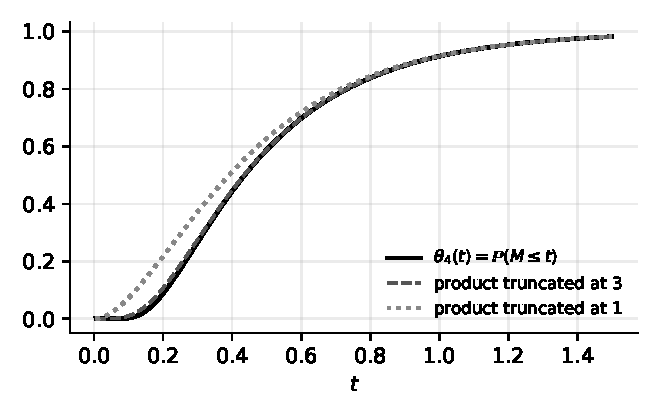
\includegraphics[width=0.6\textwidth]{fig/maxwald_maxcdf.pdf}
\caption{The distribution function $\vartheta_4$ of $M_4$, with the product of exponential distribution functions truncated after one and after three factors of each kind.}
\label{mw:fig:maxcdf}
\end{figure}

\begin{figure}[htbp]
\centering
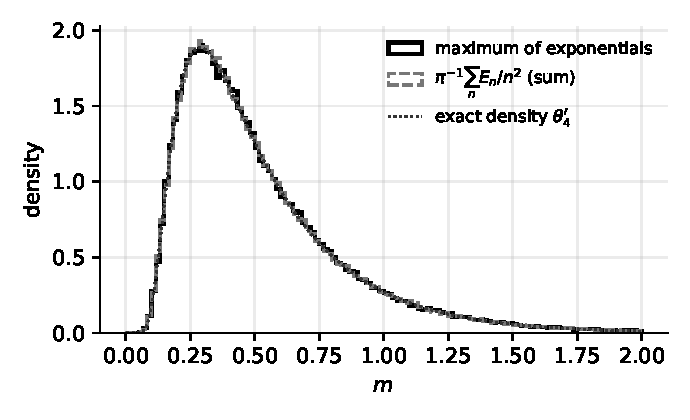
\includegraphics[width=0.62\textwidth]{fig/maxwald_mc.pdf}
\caption{Histograms of $M_4$ simulated as a maximum of exponentials and as a weighted sum of exponentials.}
\label{mw:fig:mc}
\end{figure}

\section{Khinchin: the zeta distribution inside the tilted maximum}\label{mw:sec:khinchin}

Khinchin \cite{Khinchin38} proved that for $\sigma>1$ the function $\zeta(\sigma+it)/\zeta(\sigma)$ is an infinitely divisible characteristic function; Gnedenko and Kolmogorov \cite{GnedenkoKolmogorov54} reproduce it as a worked example, and Lin and Hu \cite{LinHu01} name the law the Riemann zeta distribution. If $\Pr(N_\sigma=n)=n^{-\sigma}/\zeta(\sigma)$, the zeta distribution of Sections~\ref{rz:sec:strip} and \ref{rz:sec:levystrip}, then $\E N_\sigma^{-it}=\zeta(\sigma+it)/\zeta(\sigma)$, and the Euler product gives $N_\sigma=\prod_pp^{G_p}$ with independent geometric variables $G_p$, $\Pr(G_p=k)=(1-p^{-\sigma})p^{-k\sigma}$. Neither Khinchin nor Gnedenko worked on the zeros or on $\Xi$; the work that continues their line stays at $\sigma>1$ \cite{LinHu01,Gut06,Nakamura22}. The completed ratio $\xi(\sigma+it)/\xi(\sigma)$ is the characteristic function of the variable $V_\sigma$ of Section~\ref{bp:sec:mellin}, whose reflection $-V_\sigma$ is Nakamura's complete Riemann zeta distribution \cite{Nakamura15}, and $V_\sigma$ is quasi infinitely divisible but not infinitely divisible for $\sigma>1$ (Proposition~\ref{sb:prop:qid}). The P\'olya density, on the other hand, is not infinitely divisible, because its characteristic function $\Xi(\theta)/\Xi(0)$ has real zeros and the characteristic function of an infinitely divisible law has none; its zeros are exactly the obstruction. Section~\ref{mw:sec:exists} shows that infinite divisibility reappears, unconditionally, on the time side of the Wald couple.

\begin{theorem}\label{mw:thm:khinchin}
Fix $\sigma>1$ and let $\widetilde M_4$ have the tilted law $\Pr(\widetilde M_4\in dm)\propto m^{\sigma/2}\Pr(M_4\in dm)$. Let $K$, $N_\sigma$ and $\Gamma_{1+\sigma/2}$ be independent of each other and of $\widetilde M_4$, with $\Pr(K=k)=(1-a)a^k$ for $k\ge0$ and $a=2^{1-\sigma}$, with $N_\sigma=\prod_pp^{G_p}$ zeta distributed with parameter $\sigma$, and with $\Gamma_{1+\sigma/2}$ gamma distributed with shape $1+\sigma/2$ and scale $1$. Then
\[
\widetilde M_4\,4^{-K}\ \stackrel{d}{=}\ \frac{\Gamma_{1+\sigma/2}}{\pi N_\sigma^2}\ \stackrel{d}{=}\ \frac{\Gamma_{1+\sigma/2}}{\pi}\prod_pp^{-2G_p}.
\]
\end{theorem}

\begin{proof}
By Section~\ref{sec:maxexp:products}, $\E M_4^{s/2}=2(1-2^{1-s})\,\pi^{-s/2}\Gamma(1+\frac s2)\zeta(s)$ for every complex $s$, because $2\xi(s)/(s-1)=2\pi^{-s/2}\Gamma(1+\frac s2)\zeta(s)$. With $s=\sigma+it$, $\E\widetilde M_4^{it/2}$ is the ratio of this at $s$ and at $\sigma$, that is
\begin{multline*}
\E\widetilde M_4^{it/2}=\frac{1-ae^{-it\log2}}{1-a}\cdot\pi^{-it/2}\\
\cdot\frac{\Gamma(1+\frac{\sigma+it}2)}{\Gamma(1+\frac\sigma2)}\cdot\frac{\zeta(\sigma+it)}{\zeta(\sigma)}.
\end{multline*}
The first factor is the reciprocal of $\E e^{-itK\log2}=\E(4^{-K})^{it/2}$. The remaining factors are $\pi^{-it/2}$, $\E\Gamma_{1+\sigma/2}^{it/2}$ and $\E N_\sigma^{-it}$. Hence $\E(\widetilde M_4\,4^{-K})^{it/2}=\E\bigl(\Gamma_{1+\sigma/2}/(\pi N_\sigma^2)\bigr)^{it/2}$ for every real $t$, which is the first identity in law; the second is the Euler product.
\end{proof}

The identity is for $\widetilde M_4$ multiplied by an independent factor $4^{-K}$; it does not factor $\widetilde M_4$ itself. The factor $4^{-K}$ is the trace of $1-2^{1-s}$ and modifies only the prime $2$.

\section{The Wald couple of the maximum}\label{mw:sec:wald}

\begin{definition}\label{mw:def:wald}
A pair $(\tau,\varsigma)$ of independent variables with $\tau\ge0$ is a Wald couple if $\E e^{s\varsigma}<\infty$ and $\E e^{s\varsigma}\,\E e^{-s^2\tau/2}=1$ for all real $s$. Equivalently, with $Z$ standard normal and independent of $\tau$, the characteristic functions of $\varsigma$ and of $\sqrt\tau Z$ form a van Dantzig pair in the sense of Section~\ref{ch:clock}: $\E e^{-\theta^2\tau/2}=1/\E e^{-\theta\varsigma}$ for real $\theta$.
\end{definition}

The name comes from Wald's identity $\E\exp(sB_\tau-s^2\tau/2)=1$: if a stopping time $\tau$ of Brownian motion $B$ has $B_\tau$ independent of $\tau$ and the stopped martingales $\exp(sB_{t\wedge\tau}-s^2(t\wedge\tau)/2)$ are uniformly integrable, then $(\tau,B_\tau)$ is a Wald couple. The exit time of $(-1,1)$, with $B_\tau=\pm1$, is the prototype. Uniform integrability cannot be dropped: the hitting time of level $1$ has $B_\tau=1$, independent of $\tau$, but $\E e^{sB_\tau-s^2\tau/2}=e^{s-|s|}\ne1$ for $s<0$.

\begin{theorem}\label{mw:thm:wald}
Let $\upsilon,\upsilon_1,\upsilon_2$ be uniform on $(-1,1)$, with $\upsilon_1$ and $\upsilon_2$ independent, let $M_4'$ be an independent copy of $M_4$, and let $c=\sqrt{\pi/2}$. Then $(M_4,c\upsilon)$ and $(M_4+M_4',c(\upsilon_1+\upsilon_2))$ are Wald couples. The associated van Dantzig pairs are $(\sin ct/(ct),\ ct/\sinh ct)$ and their squares, and $\sqrt{M_4}\,Z$ has the logistic law with characteristic function $ct/\sinh ct$.
\end{theorem}

\begin{proof}
$\E e^{-s^2M_4/2}=cs/\sinh(cs)$ by Section~\ref{sec:maxexp:products}, with $\lambda=s^2/2$, and $\E e^{sc\upsilon}=\sinh(cs)/(cs)$. Squaring gives the second couple.
\end{proof}

The pair $(\sin\theta/\theta,\theta/\sinh\theta)$ is the classical van Dantzig pair of Section~\ref{ch:clock} \cite{Lukacs68}, at $\theta=ct$, and the language of Wald couples is that of the first author's \cite{P18}. The logistic statement is the representation of the logistic law as a normal scale mixture with Kolmogorov mixing of Andrews and Mallows \cite{AndrewsMallows74} and Stefanski \cite{Stefanski91}, read through the maximum: $\sqrt{M_4}$ is $\sqrt{2/\pi}$ times a variable with the Kolmogorov law, since $\pi M_4$ is twice its square.

\section{The clock exists and is infinitely divisible}\label{mw:sec:exists}

The manuscript proves that $1/G$ is the Laplace transform of a probability law by showing $(-1)^kW^{(k)}>0$ for $0\le k\le10^{10}$ from Weil's explicit formula and the verification of RH to height $3\times10^{12}$, and it reads the infinite divisibility, the self decomposability and the unimodality of the clock off the cases $k=0$ and $k=1$. The book has all of this in a stronger form, and we use it as it stands. Theorem~\ref{thm:ch12:idsd} proves unconditionally, using only the verification of RH below height $1000$, that $W>0$ and $W'<0$ on $(0,\infty)$, so that the clock is the Laplace transform of an infinitely divisible, self decomposable law with L\'evy density $W(x)/x$; the law is unimodal by Yamazato's theorem \cite{Yamazato78} (Section~\ref{ch:sato}), and its mean is $\E T=\xi''(\frac12)/(2\xi(\frac12))=0.0231050$ (Section~\ref{ch:clock}). The formulas $\log G(\lambda)=\int_0^\infty(1-e^{-\lambda x})W(x)\,x^{-1}dx$ and $(G'/G)(\lambda)=\int_0^\infty e^{-\lambda x}W(x)\,dx$, and the explicit formula for $W$ through the primes, \eqref{eq:ch2:Warith}, are in Section~\ref{ch:clock}. The ladder of signs $(-1)^kW^{(k)}>0$ is Theorem~\ref{thm:ch12:cm} for $0\le k\le10^{17}$, Theorem~\ref{thm:ch12:cmint} for every order on $(0,1.29]$ and Theorem~\ref{thm:ch12:window} for every $t>0$ and every $k\le1.16\times10^{25}$, so the range of the manuscript lies far inside that of the book. Its route takes a Cauchy circle of radius $x/2$ for the prime term and the first zero as the dominating zero. The same circle is used in the proof of Theorem~\ref{rz:thm:nmono}, where it loses a factor $2^k$ and makes the reach grow only linearly in the verified height $H$, up to a logarithm (Section~\ref{sec:ch12:reach}); from $H=3\times10^{12}$ the manuscript's constants reach orders of about $1.3\times10^{10}$, and those of that proof about $8.8\times10^{10}$ (Remark~\ref{mw:rem:orders}).

\begin{remark}\label{mw:rem:waldT}
The clock gives a Wald couple on the Riemann side: $(T,X/\sqrt2)$ is a Wald couple, equivalently the characteristic functions of $X/\sqrt2$ and of $\sqrt T\,Z$ form a van Dantzig pair. Indeed $T$ exists by Theorem~\ref{thm:ch12:idsd}, $\E e^{sX/\sqrt2}=\xi(\frac12+s/\sqrt2)/\xi(\frac12)$ and $\E e^{-s^2T/2}=\xi(\frac12)/\xi(\frac12+|s|/\sqrt2)$, and $\xi(\frac12+w)$ is even in $w$. This is the van Dantzig pair $(\Xi(\theta)/\Xi(0),\ \xi(\frac12)/\xi(\frac12+\theta))$ of Theorem~\ref{thm:ch12:idsd} read at $\theta=s/\sqrt2$, and the manuscript's $\sqrt2\,V$ is $X/\sqrt2$. Compare Theorem~\ref{mw:thm:wald}: the uniform variable with characteristic function $\sin ct/(ct)$ is replaced by the P\'olya variable, and the maximum $M_4$ by the clock. Both components exist unconditionally.
\end{remark}

\section{A Stieltjes criterion}\label{mw:sec:stieltjes}

Section~\ref{ch:ggc} reads the GGC property through the Stieltjes transform of the Thorin measure. For the clock, $G'/G=-\frac d{d\lambda}\log(1/G)$ takes the place of the function $f_H$ there, whether or not RH holds, and by Section~\ref{ch:clock} $(G'/G)(\lambda)=\sum_k(\lambda+a_k)^{-1}=\int_0^\infty e^{-\lambda x}W(x)\,dx$. The quantity of this section is
\[
r_\eta(x)=\frac1\pi\,\Im\frac{G'}{G}(-x-i\eta),\qquad x\in\R,\ \eta>0,
\]
defined wherever $-x-i\eta$ is not a pole of $G'/G$. If the clock is a GGC with Thorin measure $U$, then $r_\eta$ is the Poisson smoothing of $U$ at distance $\eta$ below the cut, as in \eqref{eq:ch3:inversion}; in the variable $-x-i\eta$ the smoothing is along horizontal lines, while the Thorin density at resolution $\varepsilon$ of Section~\ref{ch:ggc} is taken along the parabola $u=(\varepsilon-i\theta)^2$.

\begin{theorem}\label{mw:thm:stieltjes}
The following are equivalent.
\begin{enumerate}
\item[(a)] The Riemann Hypothesis.
\item[(b)] $T$ is a GGC; then $T\stackrel{d}{=}\sum_{\gamma>0}e_\gamma/\gamma^2$ and its Thorin measure is $U_{\RH}=\sum_{\gamma>0}\delta_{\gamma^2}$, the ordinates counted with multiplicity.
\item[(c)] $G'/G$ is a Stieltjes function.
\item[(d)] $r_\eta(x)\ge0$ for all $x\in\R$ and $\eta>0$ for which $-x-i\eta$ is not a pole of $G'/G$.
\item[(e)] $W$ is completely monotone.
\end{enumerate}
In that case $r_\eta$ is the Poisson smoothing of $U_{\RH}$ at scale $\eta$, and $U_{\RH}((0,x])=N(\sqrt x)$.
\end{theorem}

Items (a), (b), (c) and (e) are in the book: (a) if and only if (b) is Proposition~\ref{prop:rigid}, (b) implies (c) by the Stieltjes form of the GGC property in Section~\ref{ch:ggc}, and (b) if and only if (e) is the characterisation of a GGC by the complete monotonicity of $k$, $x$ times its L\'evy density \cite{Bondesson}, with $k=W$ for the clock (Sections~\ref{ch:clock} and \ref{ch:ggc}). The new statement is (d), the form in the variable $-x-i\eta$.

\begin{proof}
It remains to prove that (c) implies (d) and that (d) implies (a); together with (a) implies (b) implies (c) this closes the circle of implications, and (b) if and only if (e) is in the book. (c) implies (d): a Stieltjes function is analytic on $\C\setminus(-\infty,0]$ and maps the upper half plane into the closed lower half plane, and $(G'/G)(\bar\lambda)=\overline{(G'/G)(\lambda)}$, so $\Im(G'/G)(-x-i\eta)\ge0$ for $\eta>0$. (d) implies (a): if RH fails, then some zero has $\beta\ne\frac12$, and since the zeros are symmetric under $\rho\mapsto\bar\rho$ and $\rho\mapsto1-\rho$ there is a zero $\rho=\beta+i\gamma$ with $\gamma>0$ and $\beta>\frac12$; Lemma~\ref{mw:lem:detect} gives $r_\eta(x_\rho)\to-\infty$ as $\eta\uparrow b$, so $r_\eta(x_\rho)<0$ for $\eta<b$ close to $b$ and (d) fails. The last statement is \eqref{eq:ch3:inversion} and the counting formula of Section~\ref{ch:ggc} for $U_{\RH}$.
\end{proof}

\begin{lemma}[Detection]\label{mw:lem:detect}
Let $\rho=\beta+i\gamma$ be a zero of multiplicity $m$ with $\beta>\frac12$ and $\gamma>0$, put $\delta=\beta-\frac12$, and write $a_\rho=x_\rho-ib$ with $x_\rho=\gamma^2-\delta^2$ and $b=2\delta\gamma$, so that $\lambda_\rho=-a_\rho=-x_\rho+ib$. Then $r_\eta(x_\rho)\to-\infty$ as $\eta\uparrow b$. Moreover, for $0<\eta<b$ such that $-x_\rho-i\eta$ is not a pole of $G'/G$,
\[
\pi r_\eta(x_\rho)=\eta\Bigl(A_\eta-\frac{2m}{b^2-\eta^2}\Bigr),
\]
where
\[
A_\eta=\frac1\eta\sum_{\lambda_{\rho'}\ne\lambda_\rho,\bar\lambda_\rho}\Im\,\bigl(-x_\rho-i\eta-\lambda_{\rho'}\bigr)^{-1},
\]
the sum running over the zeros $\rho'$ with $\Im\rho'>0$, counted with multiplicity, whose $\lambda_{\rho'}$ is neither $\lambda_\rho$ nor $\bar\lambda_\rho$. Hence $r_\eta(x_\rho)<0$ at every $\eta\in(0,b)$ with $A_\eta<2m/b^2$. If all the other zeros lie on the line, $A_\eta\to A_0=\sum_{\gamma'}(\gamma'^2-x_\rho)^{-2}$ as $\eta\downarrow0$.
\end{lemma}

\begin{proof}
At $x=x_\rho$ we have $-x_\rho-i\eta-\lambda_\rho=-i(\eta+b)$ and $-x_\rho-i\eta-\bar\lambda_\rho=-i(\eta-b)$. Since $\Im(-iy)^{-1}=1/y$, each of the $m$ copies of the pair $\lambda_\rho,\bar\lambda_\rho$ contributes $1/(\eta+b)+1/(\eta-b)=-2\eta/(b^2-\eta^2)$, which gives the display. This tends to $-\infty$ as $\eta\uparrow b$, while all other terms stay bounded, because the other poles of $G'/G$ lie at a positive distance from $-x_\rho-ib$. If $A_\eta<2m/b^2$ then $A_\eta<2m/(b^2-\eta^2)$ for every $\eta\in(0,b)$. For a zero $\rho'$ on the line, $\lambda_{\rho'}=-\gamma'^2$ and $\Im(-x_\rho-i\eta+\gamma'^2)^{-1}=\eta/((\gamma'^2-x_\rho)^2+\eta^2)$, which gives the limit $A_0$.
\end{proof}

For $x\ne x_\rho$ the same computation shows that the $m$ copies of the pair contribute $m\,[P_{b+\eta}(x-x_\rho)-P_{b-\eta}(x-x_\rho)]$ to $r_\eta(x)$ for $0<\eta<b$, with $P_h$ the Poisson kernel of width $h$: a positive kernel of width $b+\eta$ and a negative kernel of width $b-\eta$, which becomes an atom of mass $-m$ at $x_\rho$ as $\eta\uparrow b$. This is the sense in which an off line zero is an atom of negative mass at $(x,\eta)=(x_\rho,b)$. A zero with $b<\sqrt{x_\rho}$ is therefore seen by a search over the window $\{0<\eta<\sqrt x,\ x\le X\}$ as soon as $x_\rho\le X$. The condition $b<\sqrt{x_\rho}$ is $\delta<\gamma/\sqrt{4\gamma^2+1}$, that is $\beta<1-1/(16\gamma^2)$ up to terms of higher order, and it follows from the zero free region $\beta<1-c/\log\gamma$ for $\gamma$ large \cite[Theorem 3.8]{Titchmarsh}; it does not follow from $b<\gamma$. A search that finds $r_\eta\ge0$ on the whole window therefore certifies that no such zero has $x_\rho\le X$, while a search on a grid is evidence only. Figure~\ref{mw:fig:offline} tests the detection on a model in which $G'/G$ is built from the first 60 zeros, on the grid of mesh $0.5$ in $x\in[1020,1150]$ and $0.1$ in $\eta\in[0.2,14]$: with all zeros on the line the minimum of $r_\eta$ on the grid is $1.8\times10^{-5}$, at the corner $(1150,0.2)$; after moving $\gamma_5$ to $\beta=0.6$ (so $b=6.59$) a negative region appears at $x\approx1084.7$ for $\eta$ up to $6.5$, with grid minimum $-0.735$ at $(x,\eta)=(1084.5,6.4)$ (on the finer grid of the figure, of mesh $0.125$ in $x$ and $0.05$ in $\eta\in[0.05,14]$, the two minima are $4.5\times10^{-6}$ and $-3.76$); at $x=x_\rho$ itself the value at $\eta=6.4$ is $-1.677$, and it tends to $-\infty$ as $\eta\uparrow b$, as the lemma predicts.

\begin{figure}[htbp]
\centering
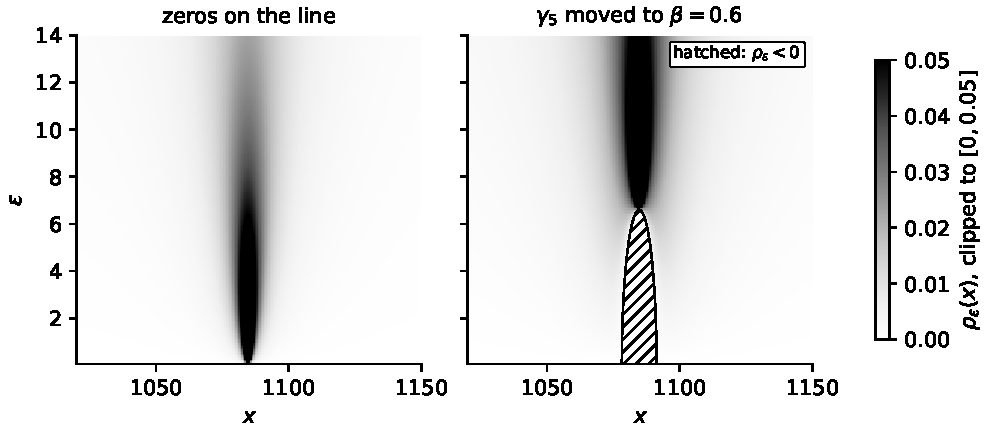
\includegraphics[width=0.86\textwidth]{fig/maxwald_offline.pdf}
\caption{The smoothed Thorin density $r_\eta(x)$ in the $(x,\eta)$ plane near $\gamma_5^2=1084.7$. Left: zeros on the line. Right: $\gamma_5$ moved off the line; the off line pair is an atom of negative mass at $(x_\rho,b)$.}
\label{mw:fig:offline}
\end{figure}
